\documentclass{article}
\usepackage[utf8]{inputenc}
\usepackage{graphicx}
\usepackage{xcolor}
\usepackage[hidelinks]{hyperref}


\definecolor{brightpink}{rgb}{1.0, 0.0, 0.5}
\definecolor{byzantine}{rgb}{0.74, 0.2, 0.64}
\definecolor{bluegray}{rgb}{0.4, 0.6, 0.8}
\definecolor{blue(ncs)}{rgb}{0.0, 0.53, 0.74}

\usepackage{helvet}
\renewcommand{\familydefault}{\sfdefault}

\setcounter{secnumdepth}{0}

\title{XRDpy User Manual}
\author{Andrew Garcia}
\date{Updated: July 2020}
  
\renewcommand*\contentsname{Summary}

\begin{document}
  
\maketitle


\tableofcontents

\pagebreak

\section{What is XRDpy?}

Github repository: \textcolor{blue(ncs)}{\textbf{\href{https://github.com/andrewrgarcia/XRDpy}{XRDpy}}} \hfill (https://github.com/andrewrgarcia/XRDpy)\\
Needed: \textcolor{blue(ncs)}{\textbf{\href{https://www.python.org/}{Python}}} \hfill (https://www.python.org/)\\
XRDpy is an XRD pattern plotting Python program which calculates crystallite size in an easy way. This program executes through the Terminal ('command line') and the execution is easy and straightforward. The program is currently divided into 2 main scripts, XRD.py and XRDsingle.py. \\\\
The first script, XRD.py, calculates the Scherrer widths for multiple XRD patterns and plots them in a single figure, where the order of the plots can be easily customized by the user through the Terminal. \\\\
The second script, XRDsingle.py, does the same but for a single XRD pattern, giving a single plot in a figure.\\\\
These scripts are currently separate of one another, but a single script integration has been entertained as it may facilitate ease of use. Nonetheless, would such be the case the functionality of the program is expected to remain the same or improve. 

\begin{figure}[htbp]
\centerline{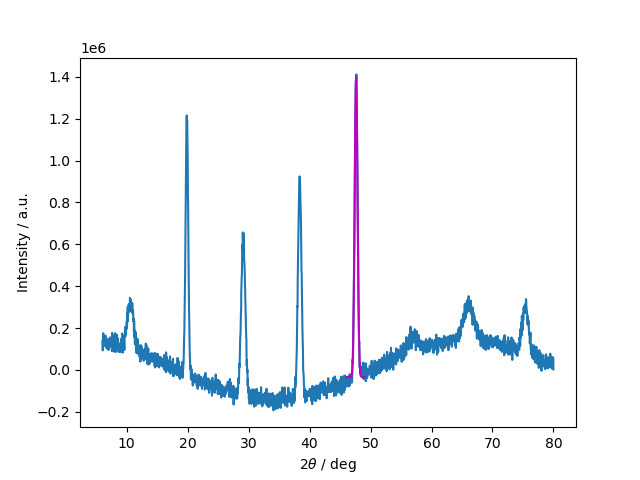
\includegraphics[scale=0.8]{intro.png}}
\caption{This is an output of the program (\textbf{python XRDsingle.py -s sample1.csv -b False -r 46 49} to be more exact).}
\label{fig}
\end{figure}

\pagebreak

\addcontentsline*{toc}{section}{}
\section{Compatibility} 

XRDpy runs on Python, which technically makes it multiplatform. However, I have only tested it in \textbf{Windows} and \textbf{Linux (Ubuntu)} operating systems, and it runs wonderfully on both. One should not find many complications running it with \textbf{Apple} systems iOS either, though the path format (directories) to access your excel and csv files may need to be changed accordingly. 

\pagebreak
\section{How do I start using it?}

Taking a pragmatic approach you may find the use of XRDpy to be very straightforward. You're encouraged to watch the instructional video of XRDpy in YouTube by \textbf{\href{https://www.youtube.com/watch?v=noYSBvC1IUQ}{clicking here}} .\\\\


\subsection{Clone the repository} 

Github repository: \textcolor{blue(ncs)}{\textbf{\href{https://github.com/andrewrgarcia/XRDpy}{XRDpy}}} \hfill (https://github.com/andrewrgarcia/XRDpy)\\
Needed: \textcolor{blue(ncs)}{\textbf{\href{git-scm.com}{Git}}} \hfill (git-scm.com)\\
Optional: \textcolor{blue(ncs)}{\textbf{\href{github.com}{Github account}}} \hfill (github.com)\\
You may need to learn the basics of Git, which aren't complicated to do. Creating a Github account will allow you to fork my repository and share any changes you may make of your forked version(s). 

\begin{description}
\item In the main XRDpy Github repository, there should be a button called "Code" or clone. Click on it and copy the HTTP address

\begin{figure}[htbp]
\centerline{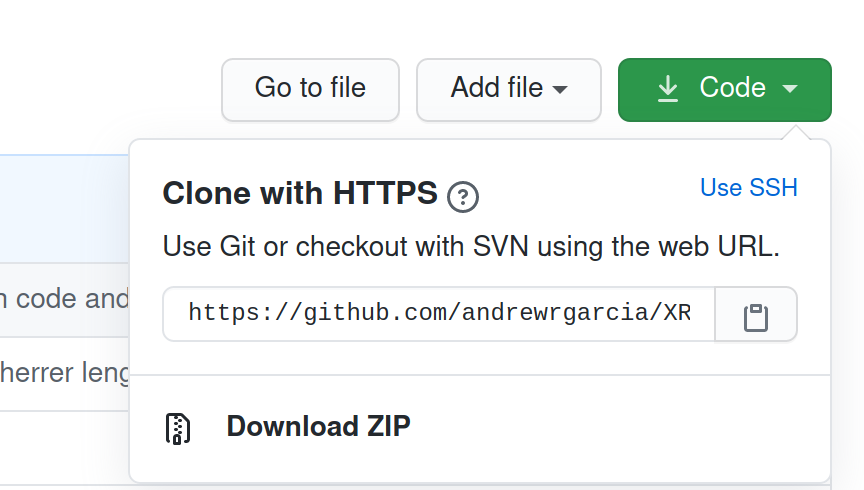
\includegraphics[scale=.35]{clone.png}}
\caption {it looks like this}
\label{fig2}
\end{figure}

\item Open your Terminal and select the folder or path where you want to place the XRDpy program (i.e. use cd command).
\item In the Terminal, type: \textbf{git clone [pasted HTTP address]}

\end{description}


\subsection{Run a simple command in the Terminal}

\begin{description}
\item Open your Terminal (or command line, or shell, whatever you call it)
\item Change to the folder containing your cloned version of XRDpy (Use the cd command to get there)
\item While in that folder, type: \textbf{python XRD.py -h}. This should bring up the lists of all the arguments available to customize and make your plot(s).

\begin{figure}[htbp]
\centerline{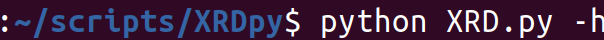
\includegraphics[scale=.35]{xrd-h.png}}
%\caption {The path to my XRDpy folder with the command from above}
\label{fig3}
\end{figure}

\end{description}


\subsection{Make your database file}

Your database file should contain the names of all your files with their .csv extension (oh yes, they should be converted or be in csv format) in the right column, as well as a short nickname in the left column that will be used to call them by the XRDpy program. Please use the \textbf{database\_template.xlsx} file provided in your cloned XRDpy folder. It makes things easier.

\begin{figure}[htbp]
\centerline{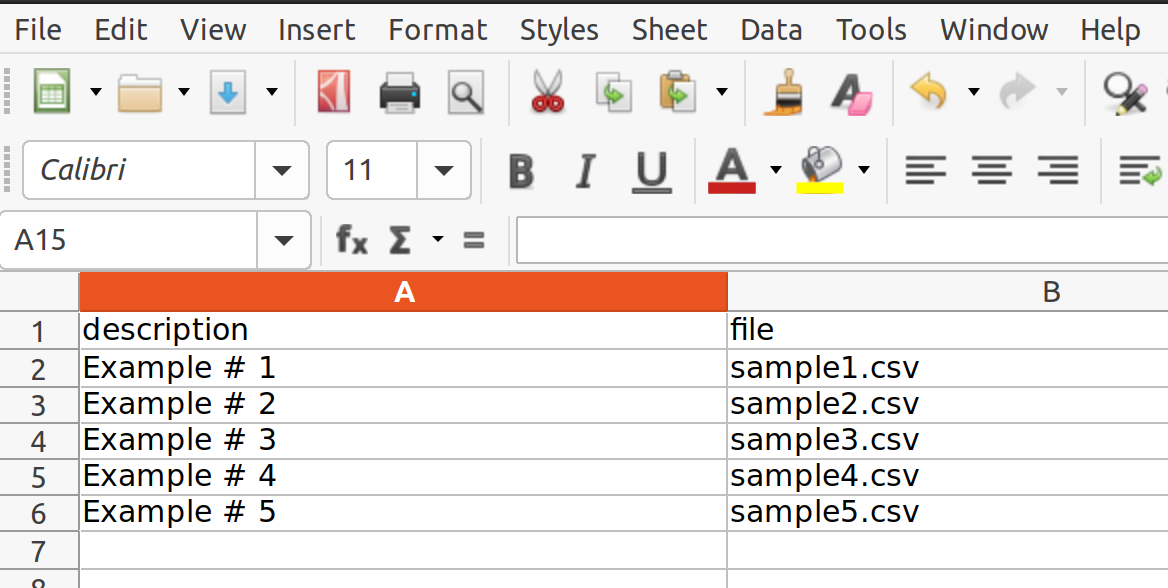
\includegraphics[scale=.2]{database-template.png}}
%\caption {If you open it, it looks like this}
\label{fig4}
\end{figure}

\subsection{Set your common XRD file directories}

\begin{figure}[htbp]
\centerline{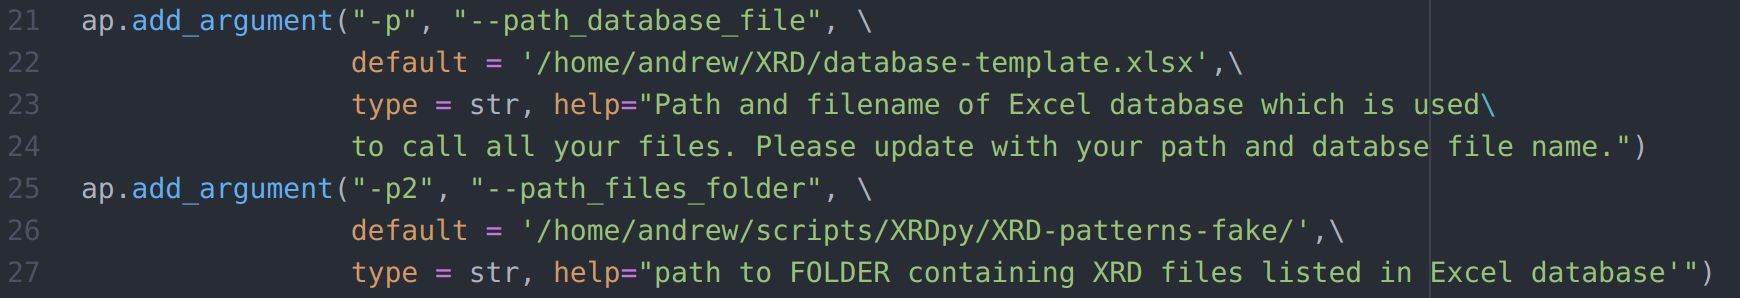
\includegraphics[scale=.27]{xrd-paths.png}}
%\caption {This is the part of the script you may want to change. Showing XRD.py here.}
\label{fig5}
\end{figure}

Open \textbf{XRD.py} and \textbf{XRDsingle.py} in a Python interpreter or text editor and change the paths where you are housing your database (see above) and your XRD files. Though you can call to switch the path in the Terminal by python XRD.py -p \textbf{['your-pathhere/.../...']} it is more efficient to have your permanent paths as defaults. \\ The argument IDs should be -p and -p2 for XRD.py and -p for XRD.single.py \\\\
For an interesting demonstration, leave the \textbf{database\_template.xlsx} file unchanged and set the -p2 path to the folder named \textbf{XRD-patterns-fake} inside your XRDpy folder


\subsection{Run XRDpy Example No. 1}

Leaving the \textbf{database\_template.xlsx} file unchanged and having set the -p2 path to the \textbf{XRD-patterns-fake} folder, type the following commands in your terminal (with the Terminal path set to the XRDpy folder): 


\begin{description}
\item \textbf{python XRD.py}    

This will display your database in the Terminal; it is an alternative to \textbf{python XRD.py -d True}. You will use the indexes from that list display and not the descriptions (i.e. use the numbers 0 1 2 3 4 in this example)

\begin{figure}[htbp]
\centerline{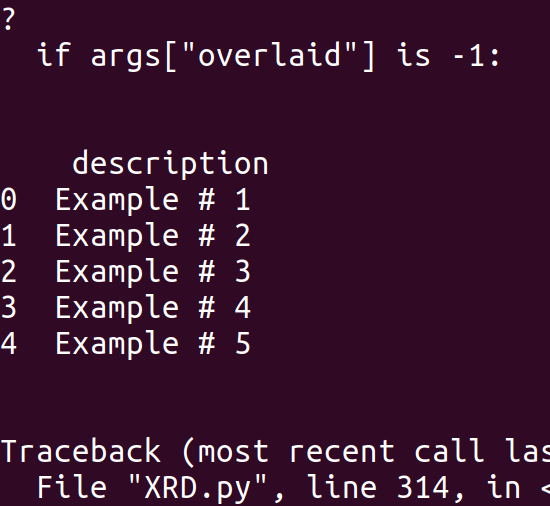
\includegraphics[scale=.3]{database-display.png}}
\caption {This is what you see. The list of the \textbf{database\_template.xlsx} file is displayed along with some silly syntax error warnings which do no harm to the development and are not even necessary in my opinion, but that's just me.}
\label{fig6}
\end{figure}

\pagebreak 

\item \textbf{python XRD.py -o 0 1 2 3 4 -x 3 2 -s 2}  

The above command will give you this plot:

\begin{figure}[htbp]
\centerline{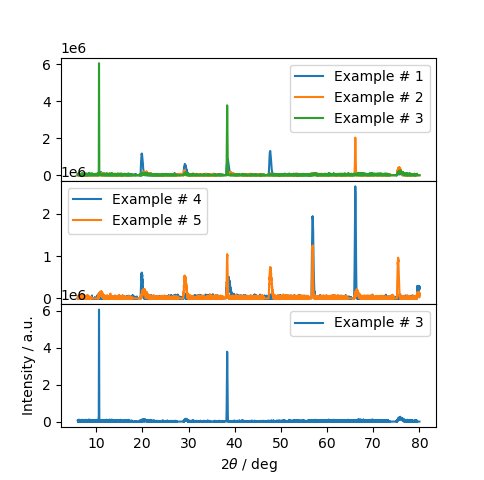
\includegraphics[scale=.70]{fake-XRDpy.png}}
\caption {\textbf{XRDpy Example No. 1} -o stands for overlaid with -x being the split of the declared overlaid plots and -s being the single plot}
\label{fig6}
\end{figure}


\end{description}

\pagebreak 

\subsection{Run XRDpy Example No. 2}

Type this in your Terminal:

\begin{description}


\item \textbf{python XRD.py -o 0 2 4 3 -x 4 -s 0 1 4 -r 36 41 -b False}  

The command plots the XRD patterns and calculates the crystallite size (Scherrer Width) for the single plots (those coming after -s); coloring the 2-$\theta$ range chosen to calculate it (here -r 36 41) in \textbf{\textcolor{byzantine}{purple}}.

\begin{figure}[htbp]
\centerline{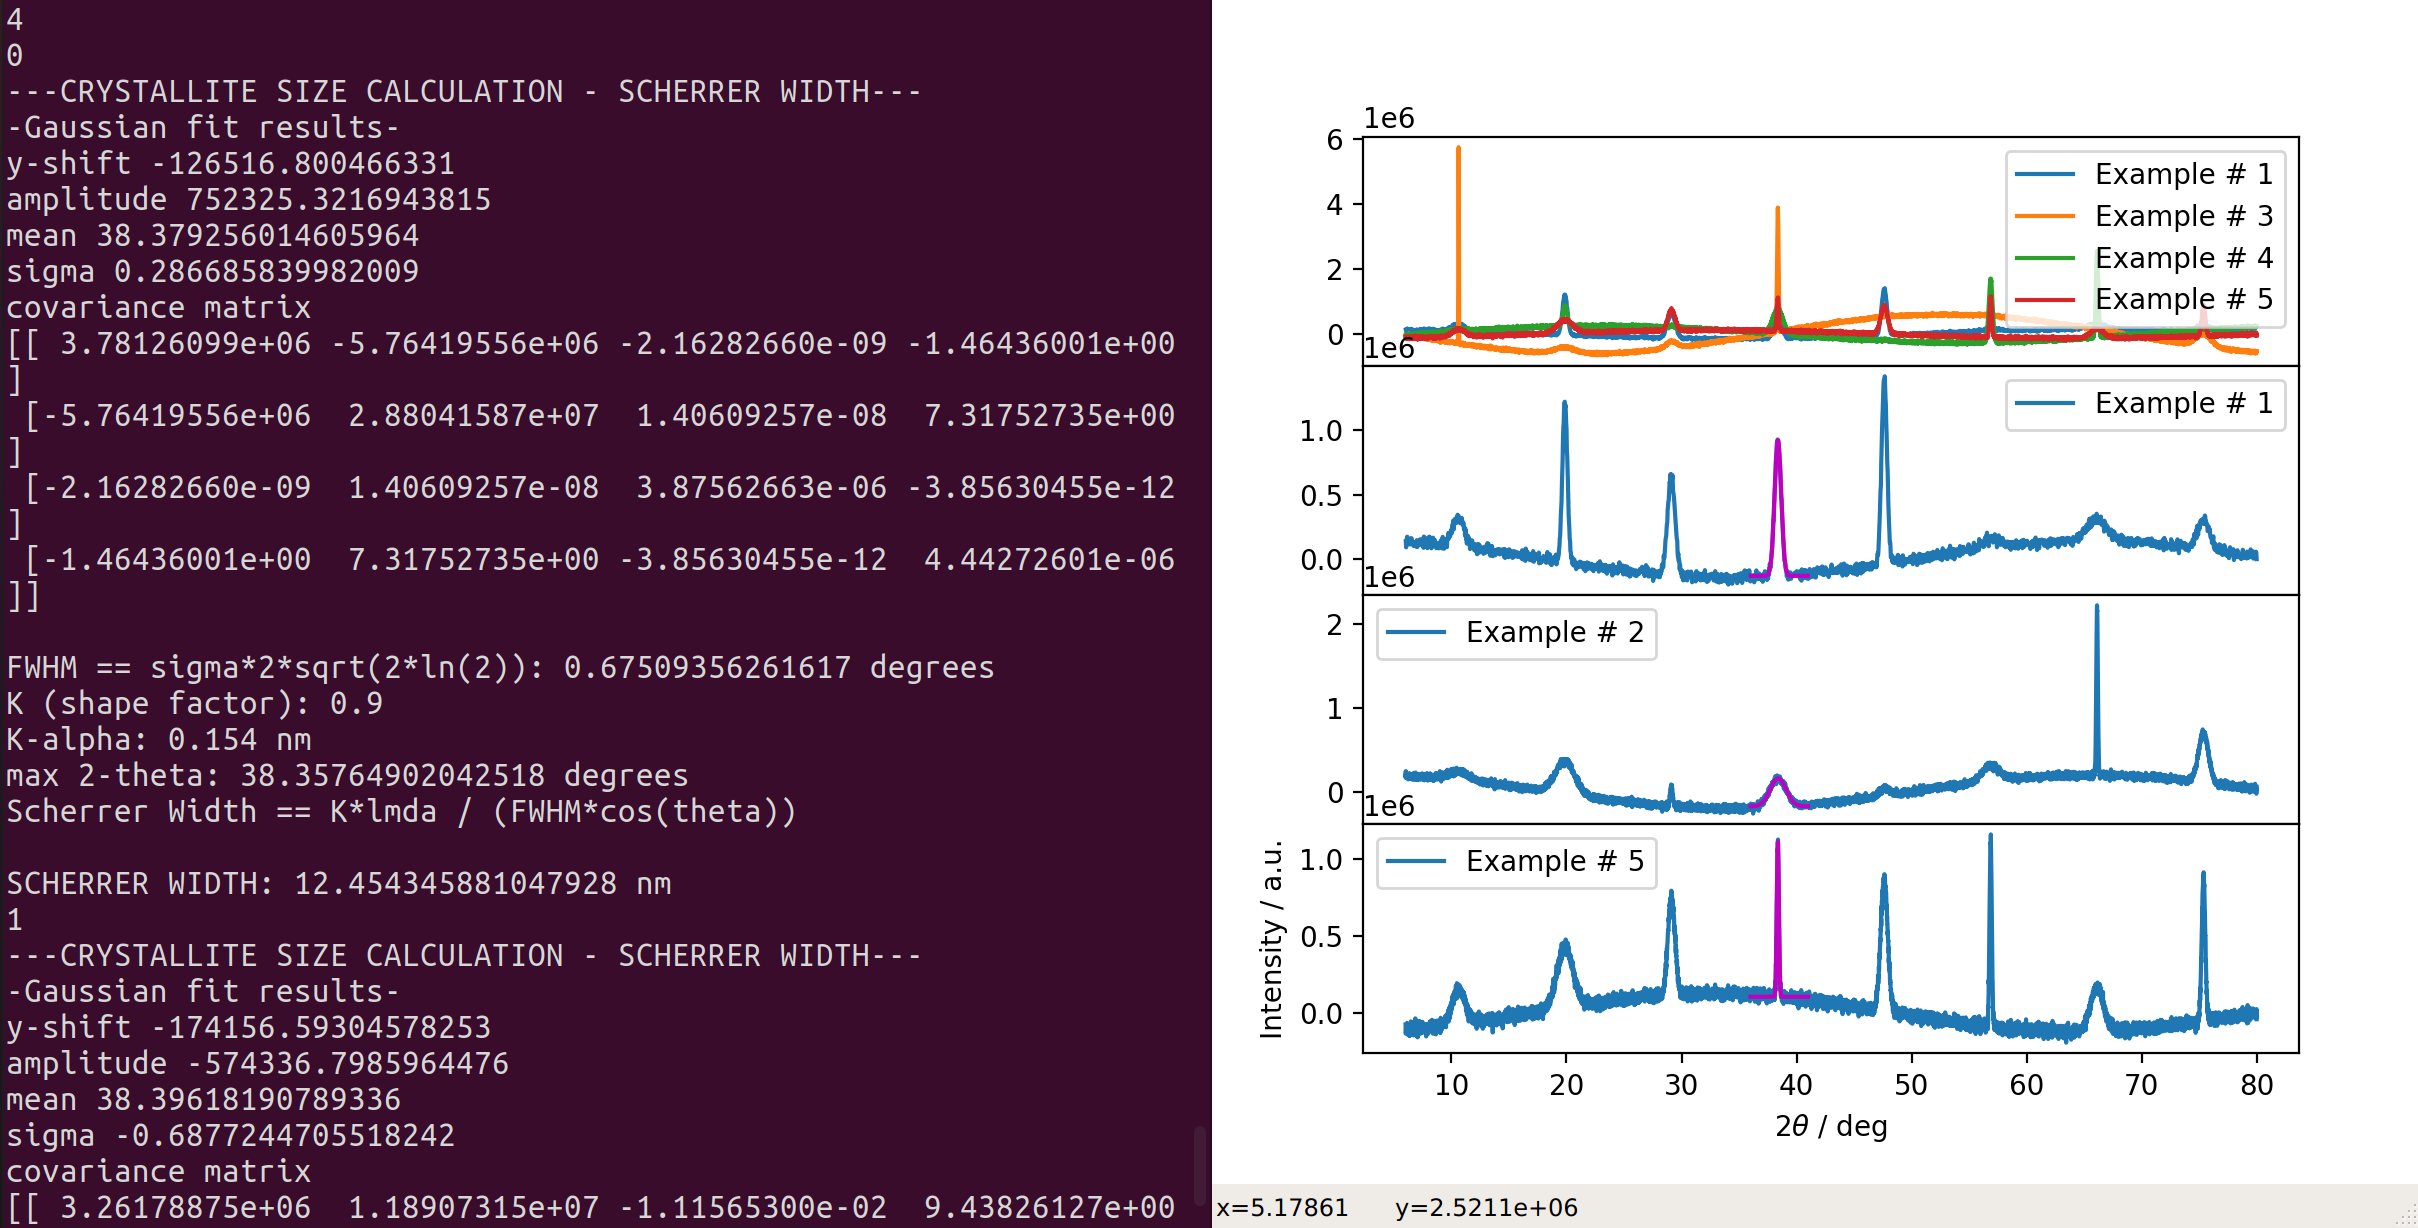
\includegraphics[scale=.2]{example-2.png}}
\caption {\textbf{XRDpy Example No. 2} -r calculates the crystallite size using the Scherrer equation at the range specified, in this case, in the range of 36 to 41 2-$\theta$; -b subtracts the background of all XRD patterns (it is set to True by default, so here I set it to False to show how the plots would look without the auto background subtraction}
\label{fig7}
\end{figure}


\end{description}

\pagebreak

\section{XRD.py arguments}

Lorem ipsum dolor sit amet, consectetuer adipiscing elit.  
Etiam lobortis facilisissem.  Nullam nec mi et neque pharetra 
sollicitudin.  Praesent imperdiet mi necante...

\subsection{-h, --help} 

Typing \textbf{python XRD.py -h} in your command prompt Terminal will give you the complete list of arguments you can run to process your XRD pattern [all the ones you see here below] . 

\subsection{-p, --path\_database\_file} 

\textcolor{brightpink}{\textbf{python XRD.py -p r'C:\textbackslash Users\textbackslash...\textbackslash database.xlsx'} \hfill	(Windows)\\
\textbf{python XRD.py -p '/home/user-name/.../database.xlsx'} \hfill (Ubuntu)}\\\\
This specifies the address and file name of your excel database of XRD patterns, where the second column displays the file names of your XRD patterns (which should be changed to .csv extensions) and the first column can be a short name you use to easily call the .csv file (see database\_template.xlsx)
For easy execution, please update the default address to your address with your excel file on the Python script and save it (line 23 XRD.py)

\subsection{-p2, --path\_files\_folder} 
\textcolor{brightpink}{\textbf{python XRD.py -p2 r'C:\textbackslash Users\textbackslash...\textbackslash XRD-files/'} \hfill  (Windows)\\\textbf{python XRD.py -p2 '/home/user-name/.../XRD-files/'}  \hfill (Ubuntu)}\\\\
This specifies the path of your folder housing all your XRD patterns which should be mentioned in your Excel database. 
For easy execution, please update the default address to your address with your excel file on the Python script and save it (line 27 XRD.py)

\subsection{-d --see\_database} 
Boolean which, when set to True, displays every common name of the XRD patterns written in your Excel database. It is defaulted to False; if you ever want to look at the contents of your database before running the plotting script, type the above underlined command. 

\subsection{-ka, --K\_alpha\_wavelength} 
This is the wavelength of K-$\alpha$ X-ray radiation, here written in units of nanometers (nm). It is defaulted to that of Copper K-$\alpha$ which corresponds to an X-ray wavelength of 0.154 nm

\subsection{-b, --background\_sub} 
This is an option to perform a baseline correction on the XRD pattern. Default is set to True, so it does it automatically. Setting it to False gives the original, uncorrected XRD pattern. 

\subsection{-o, --overlaid} 
Here is where you list all the plots you want to overlay in your figure (see Examples 1 and 2)


\subsection{-x, --overlaid\_split} 
The overlaid "split". dictates how you want to partition the overlaid plots into different sets (see Examples 1 and 2)

\subsection{-s, --single} 
List of plots you want to place separated in single charts in your figure (see Examples 1 and 2)

\subsection{-u, --units} 
The units of your x-axis. Default is set to units of 2-$\theta$ (\textbf{-u angle}). Units of interplanar spacing in nm can be set by the command \textbf{-u braggs}

\subsection{-r, --Scherrer\_range} 
Calculates crystallite size using the Scherrer equation with the specified 2-$\theta$ range input after -r (e.g. \textbf{-r 20 40} would be range from 20 to 40 2-$\theta$)

\subsection{-K, --shape\_factor\_K} 
This specifies the shape factor or "K" from the Scherrer equation. Default is set to K = 0.9

\pagebreak


\section{XRDsingle.py arguments}

\subsection{-h, --help} 

Typing \textbf{python XRD.py -h} in your command prompt Terminal will give you the complete list of arguments you can run to process your XRD pattern [all the ones you see here below] . 

\subsection{-p, --path}
\textcolor{brightpink}{\textbf{python XRD.py -p2 r'C:\textbackslash Users\textbackslash.../'} \hfill  (Windows)\\\textbf{python XRD.py -p2 '/home/user-name/.../'}  \hfill (Ubuntu)}\\\\
For \textbf{XRDsingle.py}, -p specifies the path of your folder where your chosen XRD file is. 

\subsection{-s, --file\_name}
The actual name of your chosen XRD file with its .csv extension in the end (e.g. sample-file.csv)

\subsection{-ka, --K\_alpha\_wavelength} 
This is the wavelength of K-$\alpha$ X-ray radiation, here written in units of nanometers (nm). It is defaulted to that of Copper K-$\alpha$ which corresponds to an X-ray wavelength of 0.154 nm

\subsection{-se, --second\_emission}
In XRD machinery with no secondary emission filters, extra peaks coming from such may show up. Setting this option -se True subtracts these secondary emissions with wavelength specified by -kb (see next argument)

\subsection{-kb, --K\_beta\_wavelength}
Wavelength of secondary emission to be subtracted. Default set to wavelength of K-$\beta$ radiation, 0.139 nm.

\subsection{-b, --background\_sub} 
This is an option to perform a baseline correction on the XRD pattern. Default is set to True, so it does it automatically. Setting it to False gives the original, uncorrected XRD pattern. 

\subsection{-xl, --toexcel}
Currently discontinued (obsolete). Set to False. 

\subsection{-r, --Scherrer\_range} 
Calculates crystallite size using the Scherrer equation with the specified 2-$\theta$ range input after -r (e.g. \textbf{-r 20 40} would be range from 20 to 40 2-$\theta$)

\subsection{-K, --shape\_factor\_K} 
This specifies the shape factor or "K" from the Scherrer equation. Default is set to K = 0.9

               
         
\end{document}

